\paragraph{Aufgabe 13}


\subparagraph{a) und b)}
Für die Teilaufgabe \textbf{b)} ergibt sich das in \ref{fig:13ab} zu sehende Histogramm.
\begin{figure}[H]
  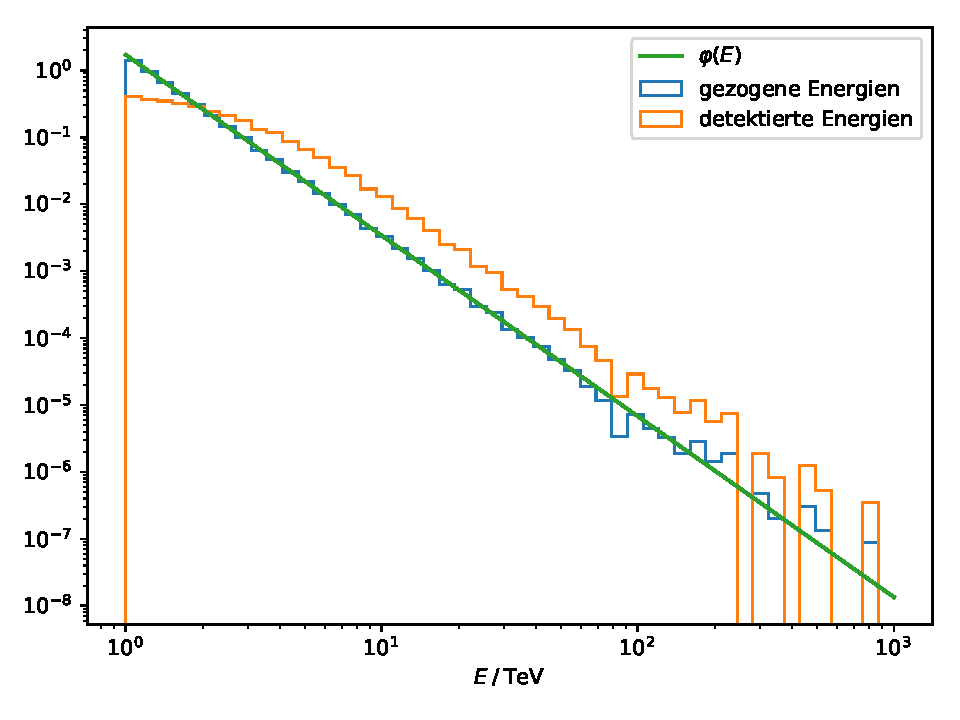
\includegraphics{Aufgabe13/b.pdf}
  \caption{Histogramm der gezogenen und detektiertenEnergien }
  \label{fig:13ab}
\end{figure}

\subparagraph{c) und d)}
 Mit den in \textit{c)} erzeugten, normalverteilten Hits folgt das in \ref{fig:13cd} zu sehende \textit{2D-Histogramm} für die gemessenden Ereignisse auf einem quadratischen Detektor.
 \begin{figure}[H]
   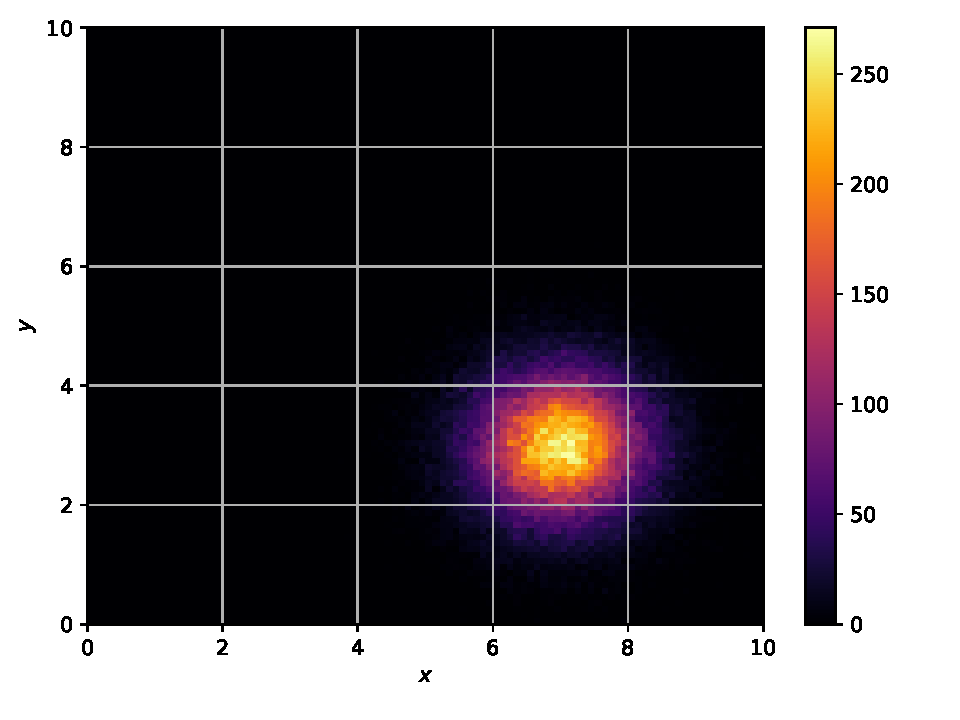
\includegraphics{Aufgabe13/d.pdf}
   \caption{Histogramm der gemessenen Ereignisse auf einem quadratischen Detektor }
   \label{fig:13cd}
 \end{figure}

 \subparagraph{e)}
 Für den Logarithmus der Anzahl der Hits folgt das in \ref{fig:13ehits} zu sehende \textit{Histogramm}.
 \begin{figure}[H]
   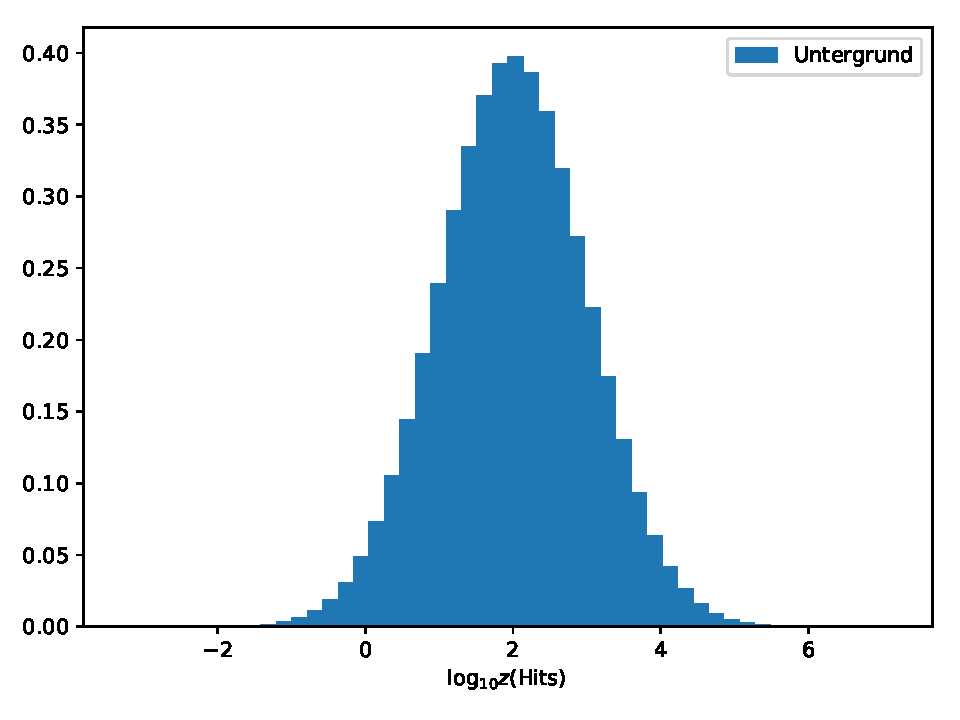
\includegraphics{Aufgabe13/e_hits.pdf}
   \caption{Histogramm für für Logarithmus der Anzahl der Hits}
   \label{fig:13ehits}
 \end{figure}
 Für die Orte der Untergrundereignisse folgt das in \ref{fig:13edetektor} zu sehende \textit{2D-Histogramm}.
 \begin{figure}[H]
   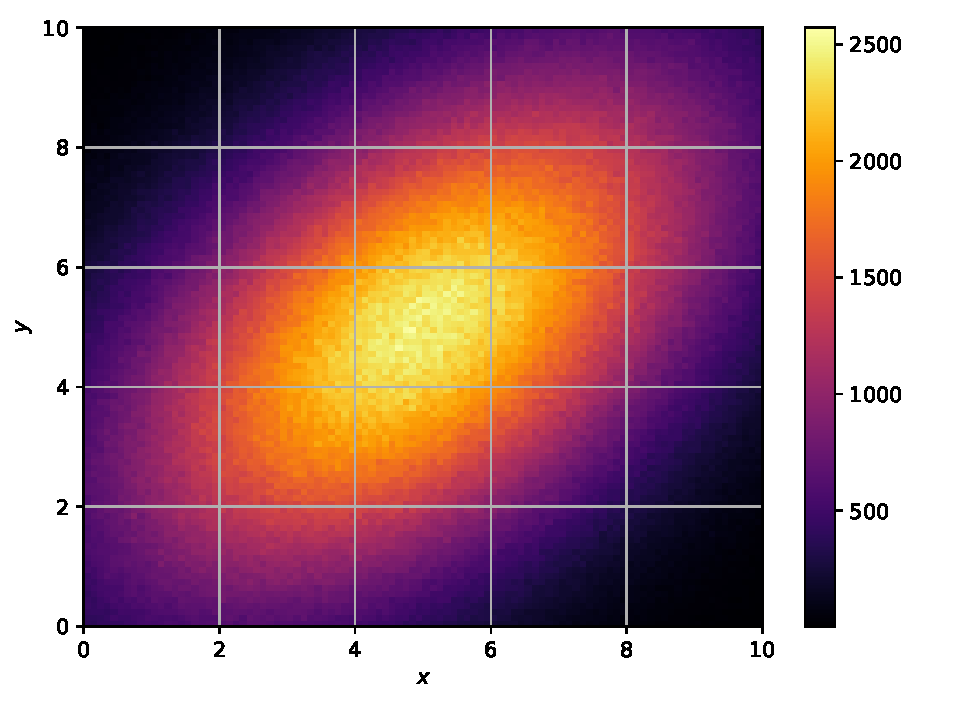
\includegraphics{Aufgabe13/e_detektor.pdf}
   \caption{Histogramm für für Logarithmus der Anzahl der Hits}
   \label{fig:13edetektor}
 \end{figure}
